\section{Algorithms}
\label{sec:algorithms}
In recent years, methods of meta learning have emerged one after another. Previous% [77], [78]
categorizations of meta-learning methods tend to produce a three-way taxonomy across optimization-based methods, model-based (or black box) methods, and metric-based (or non-parametric) methods.
Today we mainly introduce the most famous example of optimization-based methods, MAML, which is to learn a good initialization for the parameters, and then use a small amount of updates to train new tasks on the basis of this initialization.

\subsection{MAML}
According to the above introduction, we can realize that: From a macro perspective, meta learning uses tasks as ``samples" for learning. So in general, we will divide the data into $Meta\_train$ and $Meta\_test$, where $Meta\_train$ contains data from multiple tasks, and can be divided into $D\_train$ and $D\_test$, which are used for training and testing respectively.

Since current machine learning methods all perform gradient updates, and the focus of MAML is on gradient updates, it can also be regarded as a gradient-based meta learning method.

The core idea of MAML is actually very simple. In each iteration step, there will be an initial parameter $\theta$, which is used to update the gradient of $K$ tasks in $D\_train$ and achieve new $\theta'_i$ of different tasks. After all $\theta'_i$ optimized on $D\_train$, we update the global parameter $\theta$ on K tasks in $D\_test$(see Figure~\ref{fig:graph}).

\begin{figure}[h]
  \centering
  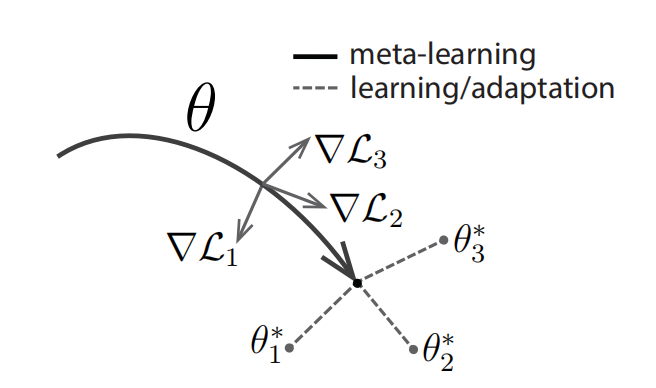
\includegraphics[totalheight=1.5in]{fig1.png}
  \caption{Diagram of our model-agnostic meta-learning algorithm (MAML)} \label{fig:graph}
\end{figure}

The gray branch lines in the figure represent the update direction of $\theta$ on different tasks, and the black line represents the final optimization of the model parameters, which can prevent the parameters from overfitting on a certain task. The last dotted lines represent processes of adaptation to new tasks, which is referred to as the fine-tune of the model parameters.

The gradient-based solution is adaptive to different kinds of learning tasks. Algorithm \ref{MAML} is the generalization of this model.



\begin{algorithm}[h]
  \caption{Model-Agnostic Meta-Learning}
  \label{MAML}
  \begin{algorithmic}[1]
    \REQUIRE $p(\mathcal{T})$: distribution over tasks
    \REQUIRE $\alpha, \beta$: step size hyperparameters
    \STATE randomly initialize $\theta$
    \WHILE {not done}
    \STATE Sample batch of tasks $\mathcal{T}_i \sim p(\mathcal{T})$
    \FORALL {$\mathcal{T}_i$}
    \STATE Evaluate $\nabla_\theta \mathcal{L}_{\mathcal{T}_i} (f_\theta)$ with respect to $K$ examples
    \STATE Compute adapted parameters with gradient descent: $\theta'_i = \theta - \alpha\nabla_\theta \mathcal{L}_{\mathcal{T}_i} (f_\theta)$
    \ENDFOR
    \STATE Update $\theta \leftarrow \theta - \beta\nabla_\theta \Sigma_{\mathcal{T}_i \sim p(\mathcal{T})}\mathcal{L}_{\mathcal{T}_i} (f_{\theta'_i})$
    \ENDWHILE
  \end{algorithmic}
\end{algorithm}

At first, we sample several tasks randomly into a batch. From step 4 to step 7, we update the parameter vector $\theta'_i$ of the model separately on support set($D\_train$) of each task in the batch using one or more gradient descent updates on task $\mathcal{T}_i$.
While using multiple gradient updates is a straightforward extension, for simplicity of notation, we use one gradient update,
$$\theta'_i = \theta - \alpha\nabla_\theta \mathcal{L}_{\mathcal{T}_i} (f_\theta).$$
The step size $\alpha$ there can be a fixed hyperparameter or a meta-learned paramter. Loss function may be MSE in regression model or cross-entropy in classification.

After that, we need to compute the second gradient update, known as meta update, on the model parameters $\theta$ using the updated parameter vector $\theta'$. We no longer use the loss of each task to update the gradient, but like common model training process, optimizing for the performance of $f_{\theta'_i}$ with respect to $\theta$ across tasks sampled from
$p(\mathcal{T})$. More concretely, the meta-objective is as follows:
$$\min_\theta \Sigma_{\mathcal{T}_i \sim p(\mathcal{T})}\mathcal{L}_{\mathcal{T}_i} (f_{\theta'_i}) = \Sigma_{\mathcal{T}_i \sim p(\mathcal{T})}\mathcal{L}_{\mathcal{T}_i} (f_{\theta - \alpha\nabla_\theta \mathcal{L}_{\mathcal{T}_i} (f_\theta)})$$
The meta-optimization across tasks is performed via
stochastic gradient descent (SGD), such that the model parameters $\theta$ are updated as follows:
$$\theta \leftarrow \theta - \beta\nabla_\theta \Sigma_{\mathcal{T}_i \sim p(\mathcal{T})}\mathcal{L}_{\mathcal{T}_i} (f_{\theta'_i})$$

The second gradient update is performed on the query set($D\_test$) in the task, which enhances the generalization of this model and avoids overfitting the support set($D\_train$).

% \begin{algorithm}
%   \caption{MAML for Few-Shot Supervised Learning}
%   \label{MAML}
%   \begin{algorithmic}[1]
%     \REQUIRE $p(\mathcal{T})$: distribution over tasks
%     \REQUIRE $\alpha, \beta$: step size hyperparameters
%     \STATE randomly initialize $\theta$
%     \WHILE {not done}
%     \STATE Sample batch of tasks $\mathcal{T}_i \sim p(\mathcal{T})$
%     \FORALL {$\mathcal{T}_i$}
%     \STATE Sample $K$ datapoints $\mathcal{D}=\{x^{(j)}, y^{(j)}\}$ from $\mathcal{T}_i$
%     \STATE Evaluate $\nabla_\theta \mathcal{L}_{\mathcal{T}_i} (f_\theta)$ with respect to $K$ examples
%     \STATE Compute adapted parameters with gradient descent: $\theta'_i = \theta - \alpha\nabla_\theta \mathcal{L}_{\mathcal{T}_i} (f_\theta)$
%     \STATE Sample datapoints $D'_i=\{x^{(j)}, y^{(j)}\}$ from $\mathcal{T}_i$ for the meta-update
%     \ENDFOR
%     \STATE Update $\theta \leftarrow \theta - \beta\nabla_\theta \Sigma_{\mathcal{T}_i \sim p(\mathcal{T})}\mathcal{L}_{\mathcal{T}_i} (f_{\theta'_i})$
%     \ENDWHILE
%   \end{algorithmic}
% \end{algorithm}